
\documentclass{article}

\usepackage{amssymb,amsmath}

\usepackage{graphicx}

\begin{document}

\section{Risk Model}

Risk is modelled as a function, $\mathbb{R}^3 \rightarrow [0, 1]$ which is use
to determine the risk at every $(x, y, z)$ location within the search space. In
order to determine risk in 3-space, we obtain a 2-D risk model which models the
risk at the minimum altitude. This function $R_0 : \mathbb{R}^2 \rightarrow [0,
1]$ determines what the risk would be at the minimum altitude. This is assumed
to be given to the algorithm \emph{a priori} or can be determined at any time
during the iteration of the algorithm. This ground risk, $R_0$, is modelled as
a lookup table rather than a combination of basis functions in order to give a
more generic model for risk that can be used in any use case of the algorithm.
To determine the 3-D risk, $R(x, y, z)$, we perform an exponential decay on the
given ground risk value, $R_0(x, y)$. 3D risk is defined as follows:

$$ R(x, y, z) = R_0(x, y) \cdot \exp{\left(-\frac{z^2}{K \cdot R_0(x,
y)^2}\right)}$$

Even though risk in 3D is evaluated and is not simply a lookup table, one can
be used instead. This representation for 3D risk is ideal for modelling fires,
detection by hostile agents, or any stimuli that would decrease monotonically
as the altitude increases.

For the experiments, we have used nine different scenes for the representation
of the ground risk, $R_0$. To generate these scenes, we used the diamond-square
algorithm~\cite{DBLP:journals/cacm/FournierFC82} to generate random terrain
maps that have values from zero to one.  The diamond-square algorithm generates
realistic random risk scenes that represent the 2D ground level risk as
anticipated. Random terrain maps have also been used
in~\cite{DBLP:conf/icra/MurphyN11} to represent random risk for path planning
problems. A heat-map showing a random terrain map generated with the diamond
square algorithm is shown in Fig~\ref{fig:risk}.

\begin{figure}[h]

    \centering

    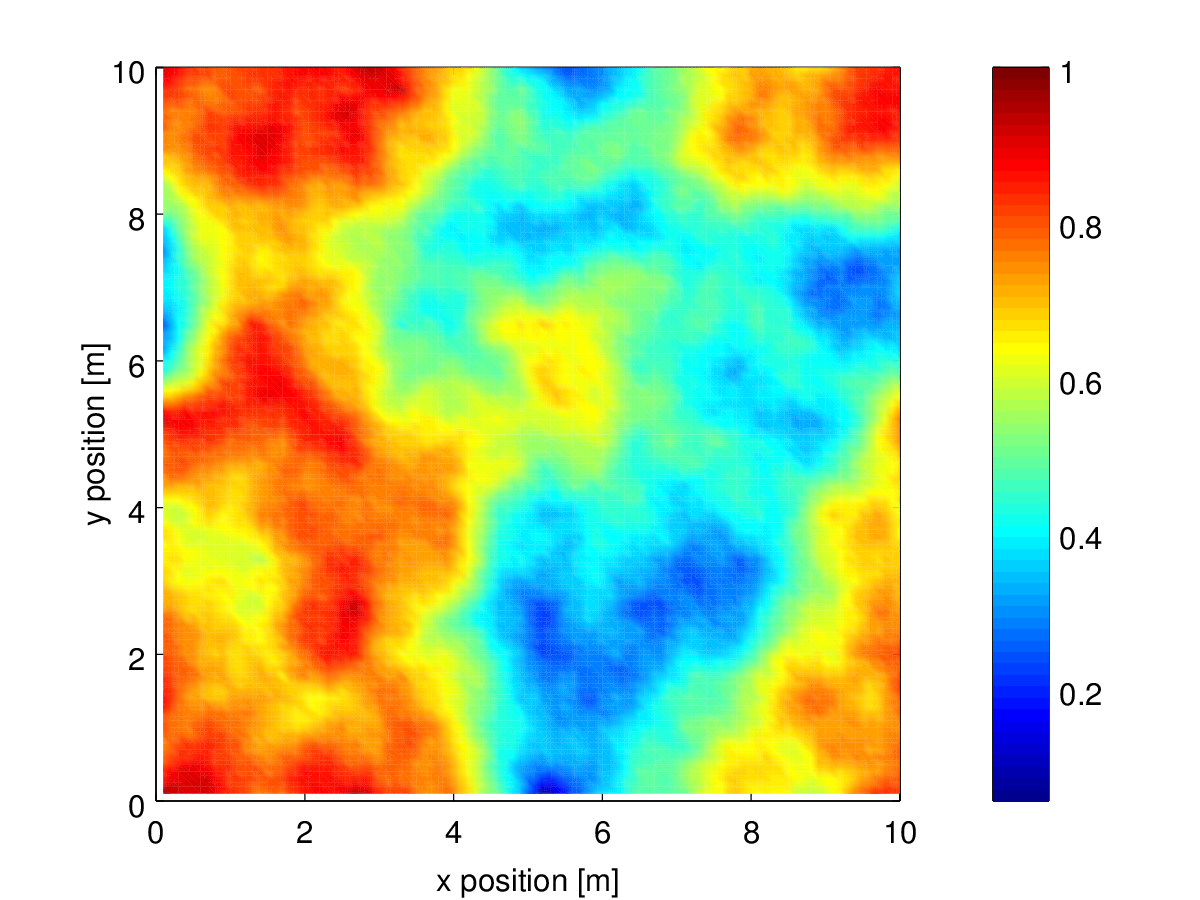
\includegraphics[width=1.0\columnwidth]{tasefigs/risk.png}

    \caption{A visualization of the ground risk, $R_0$}

    \label{fig:risk}

\end{figure}

\section{2D Planning}

Quadrotors use a very simple, reactive rule to determine where to move that has
extremely emergent properties.  Given a map, $M$, quadrotors move to areas with
a combination of the largest uncertainty, $\Upsilon$, and the lowest risk, $R$.
Our implementation uses a cost surface that is shared between members of the
swarm. Since the quadrotors update this cost surface as they move around it,
the cost surface is used as the mode of communication between the quadrotors.
This cost surface removes the need for the agents to have any peer to peer
communication and also removes the need for any agent to have perfect
information about the swarm.

For a quadrotor to determine a new heading, the agent samples costs from the
surface around the edge of its sensor foot print. It then moves in the
direction of the smallest cost. One it has moved, the agent updates the
measurements for the uncertainty grid, $\Upsilon$ for the area that was just
covered in by the sensor foot print. This uncertainty update happens
iteratively in the swarm, so the quadrotors left the plan their movements have
an updated grid before they determine a new heading.

The cost surface, $\Gamma$, is made up of a combination of the uncertainty
grid, $\Upsilon$ and the risk surface of the region. More formally, assume that
there is a function $\delta : \mathbb{R}^2 \rightarrow \mathbb{R}$ which is
used to combine the uncertainty and risk into one metric. This is assumed to be
a user defined function which may change from application to application. The
cost surface is then defined as,

$$\Gamma(x, y) = \delta(\Upsilon(x, y), R(x, y))$$

For our implementation we defined $\delta$ as,

$$\delta(\upsilon, r) = \max{\Upsilon} - \upsilon + 100 \cdot r$$

An instance of the uncertainty surface, $\Upsilon$, is shown in
Fig~\ref{fig:cost} where the $x, y$ coordinate represents the 2D position within
the workspace and the color represents the level of uncertainty. Notice the two
dark blue ellipses with low uncertainty. That is the current sensor footprint
of the quadrotors at the time at which the snapshot was taken.
Fig.~\ref{fig:cost} shows a snapshot of the cost surface which is created by
combining the risk surface shown in Fig.~\ref{fig:risk} and the uncertainty
surface shown in Fig.~\ref{fig:cost} using the $\delta$ combination function
used in our implementation.

\begin{figure}[h!]

    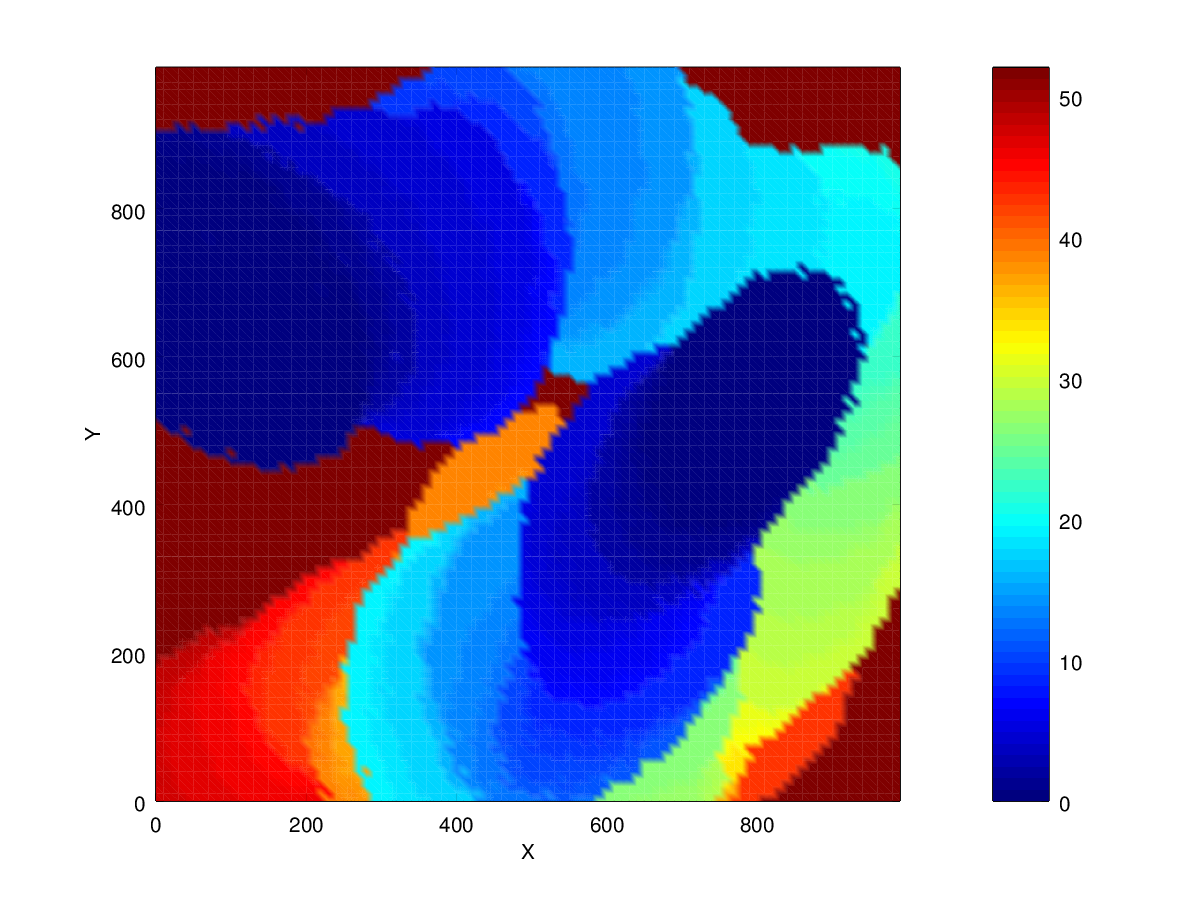
\includegraphics[width=0.49\columnwidth]{tasefigs/grid3.png}
    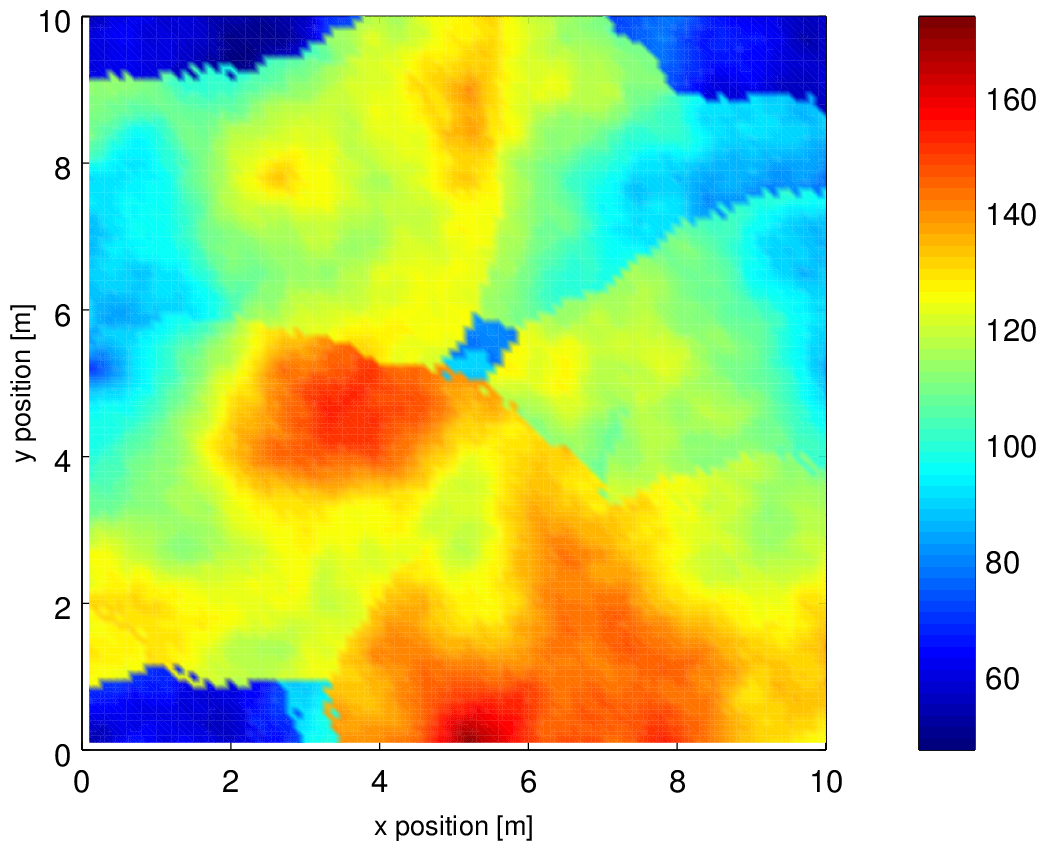
\includegraphics[width=0.49\columnwidth]{tasefigs/cost3.png}

    \caption{The two images show the uncertainty surface and the cost surface
    respectively. The cost surface is a combination of the risk shown in
    Fig.~\ref{fig:risk} and the uncertainty surface.}

    \label{fig:cost}

\end{figure}

Fig.~\ref{fig:together} shows snapshots of the algorithm in sequence. The
figures show iteration 1, 25, 50, and 100. These figures show the
representation of the uncertainty surface and the cost surface. As the
algorithm progresses the uncertainty of the area changes and so does the
associated cost. These surfaces are vital for the planning of the quadrotors.

\begin{figure}[ht]

    \centering
    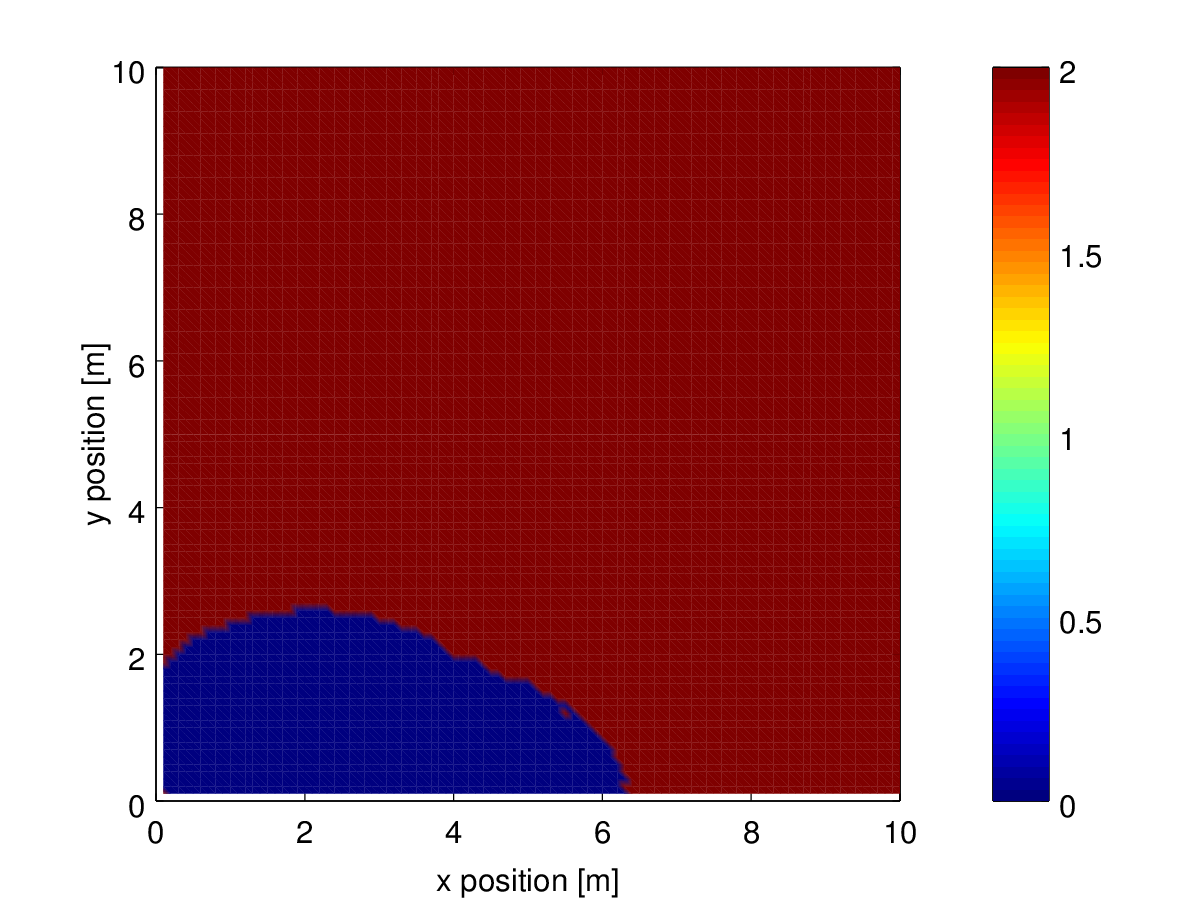
\includegraphics[width=0.24\linewidth]{tasefigs/grid1.png}
    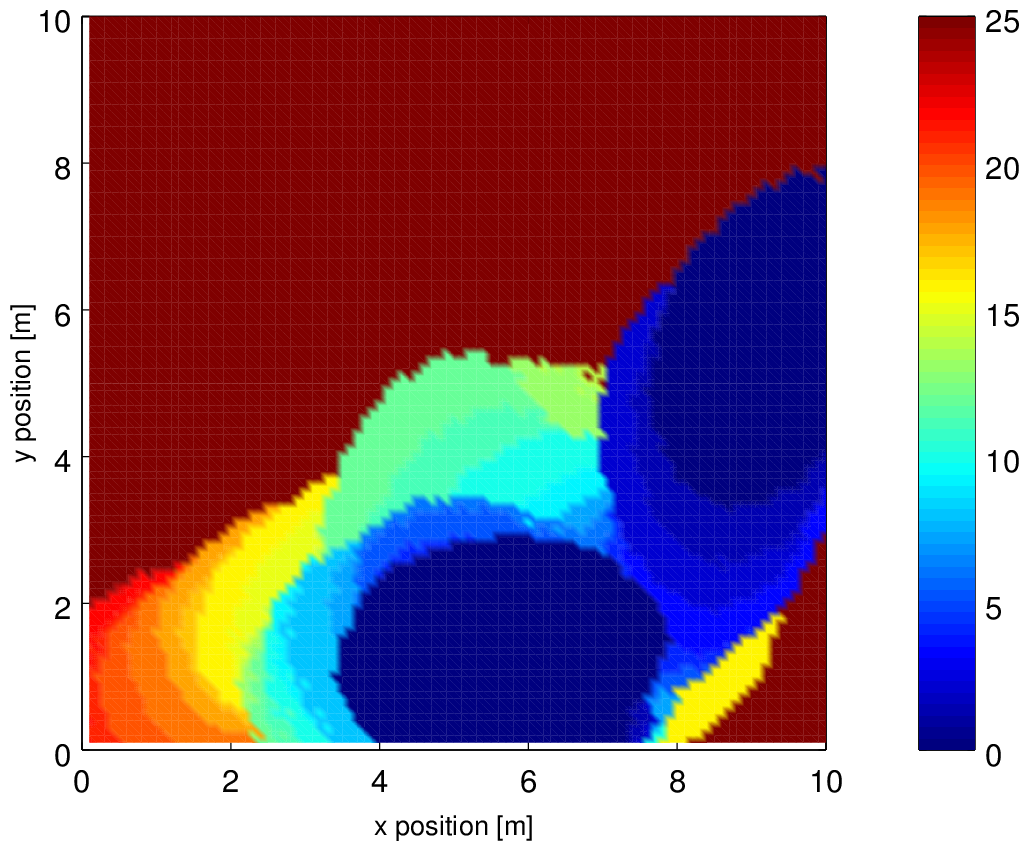
\includegraphics[width=0.24\linewidth]{tasefigs/grid2.png}
    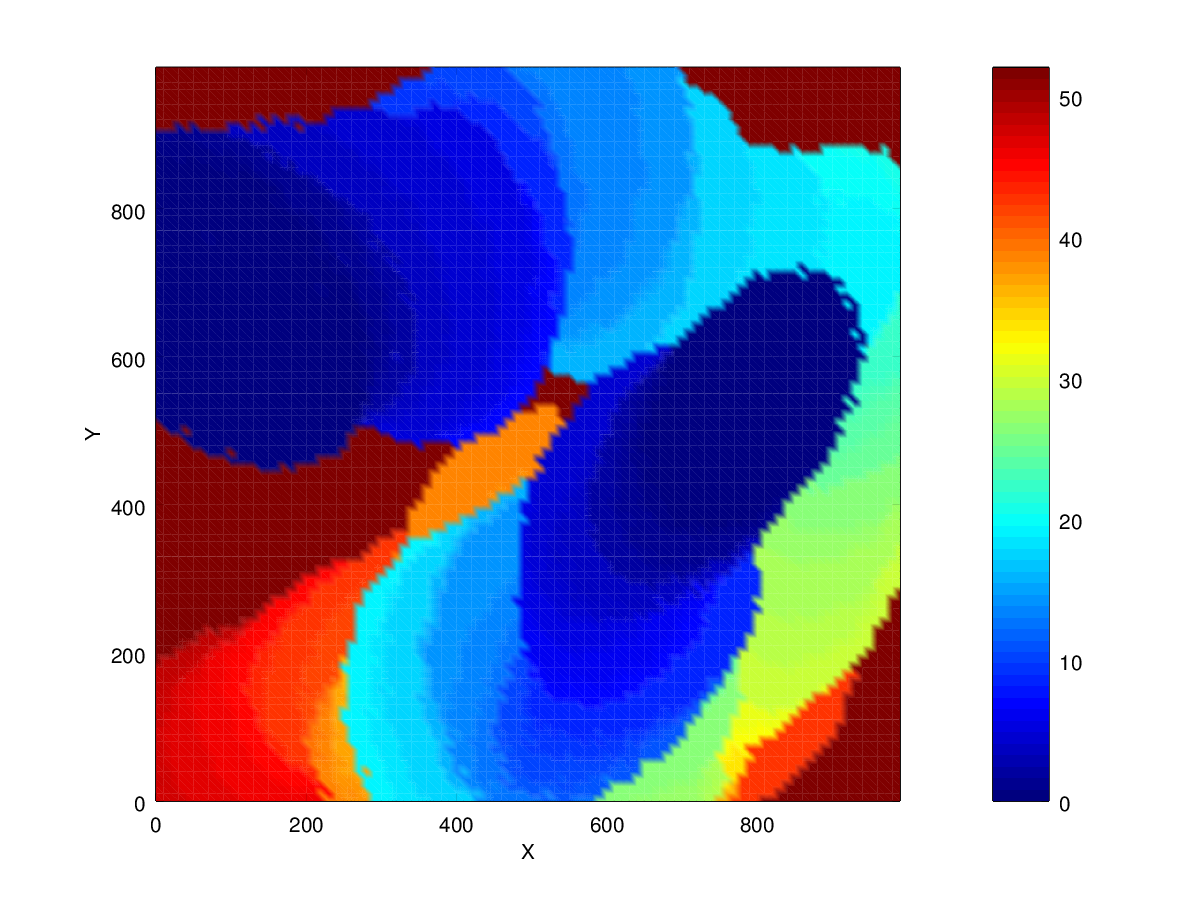
\includegraphics[width=0.24\linewidth]{tasefigs/grid3.png}
    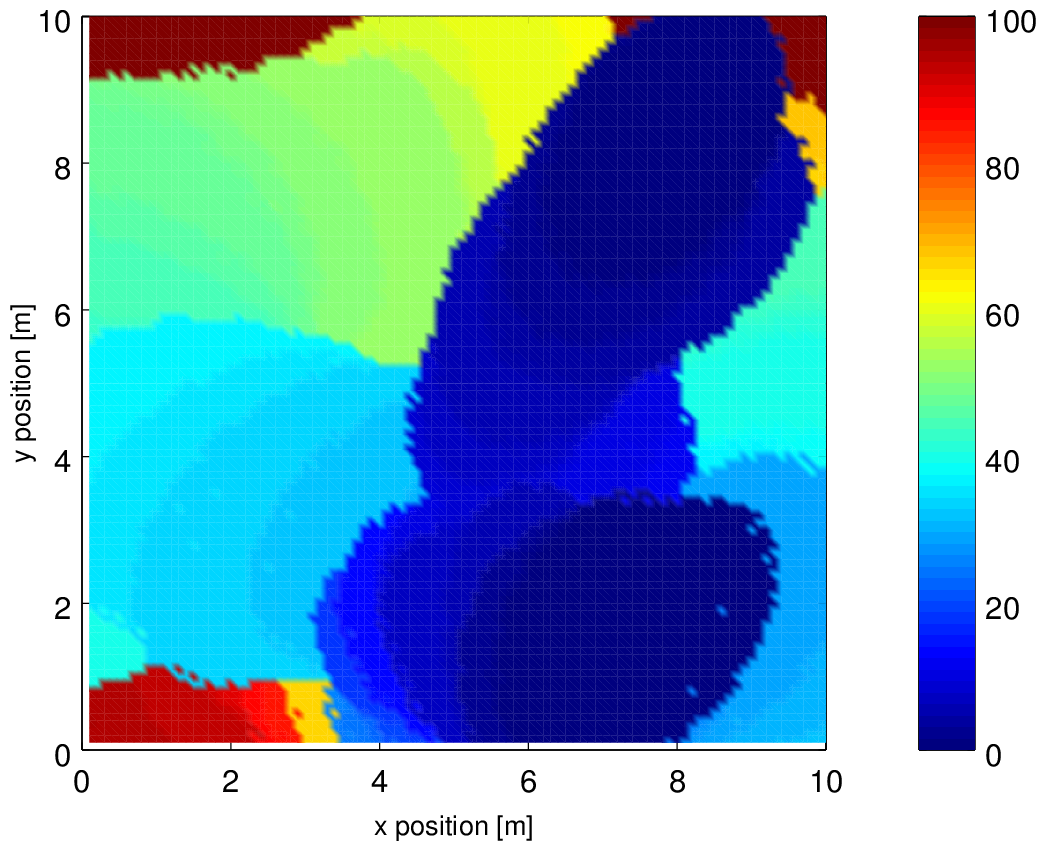
\includegraphics[width=0.24\linewidth]{tasefigs/grid4.png} \\
    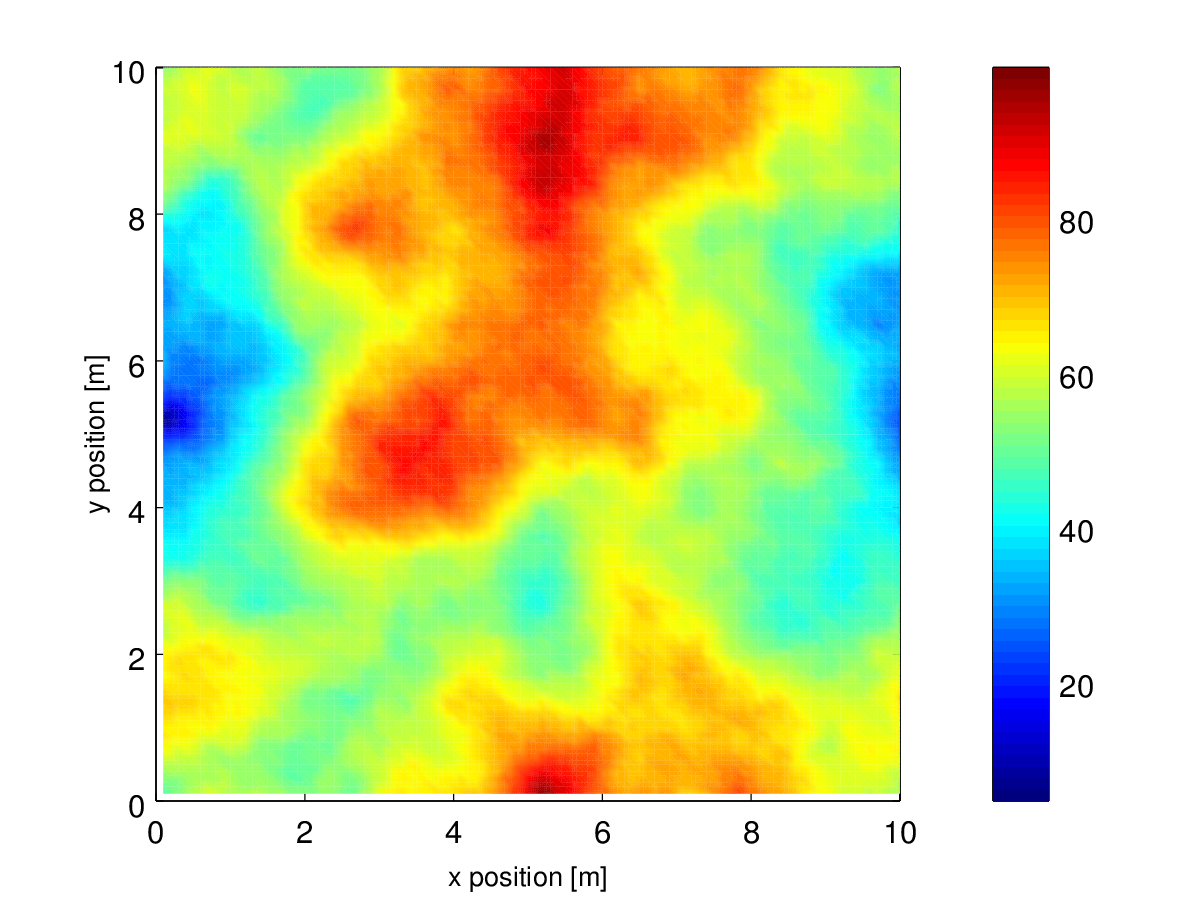
\includegraphics[width=0.24\linewidth]{tasefigs/cost1.png}
    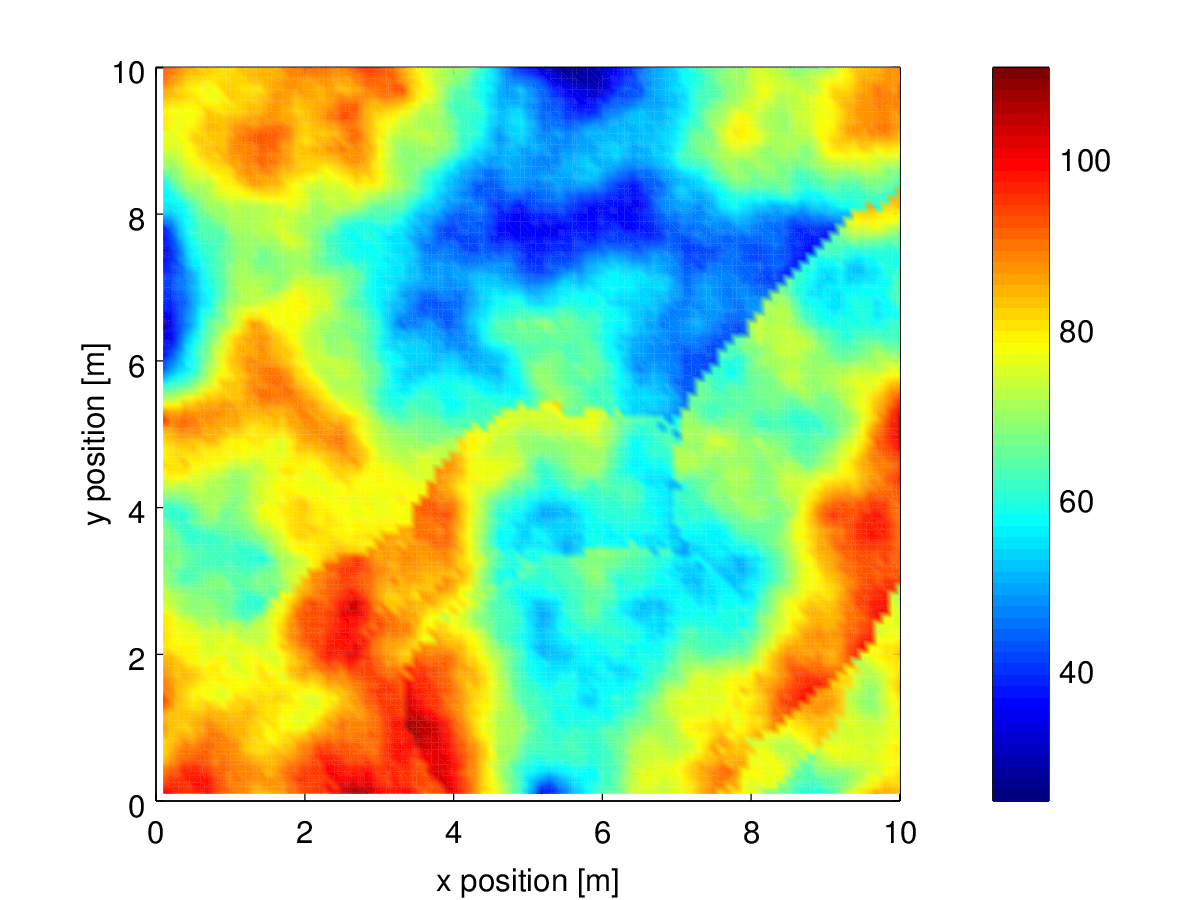
\includegraphics[width=0.24\linewidth]{tasefigs/cost2.png}
    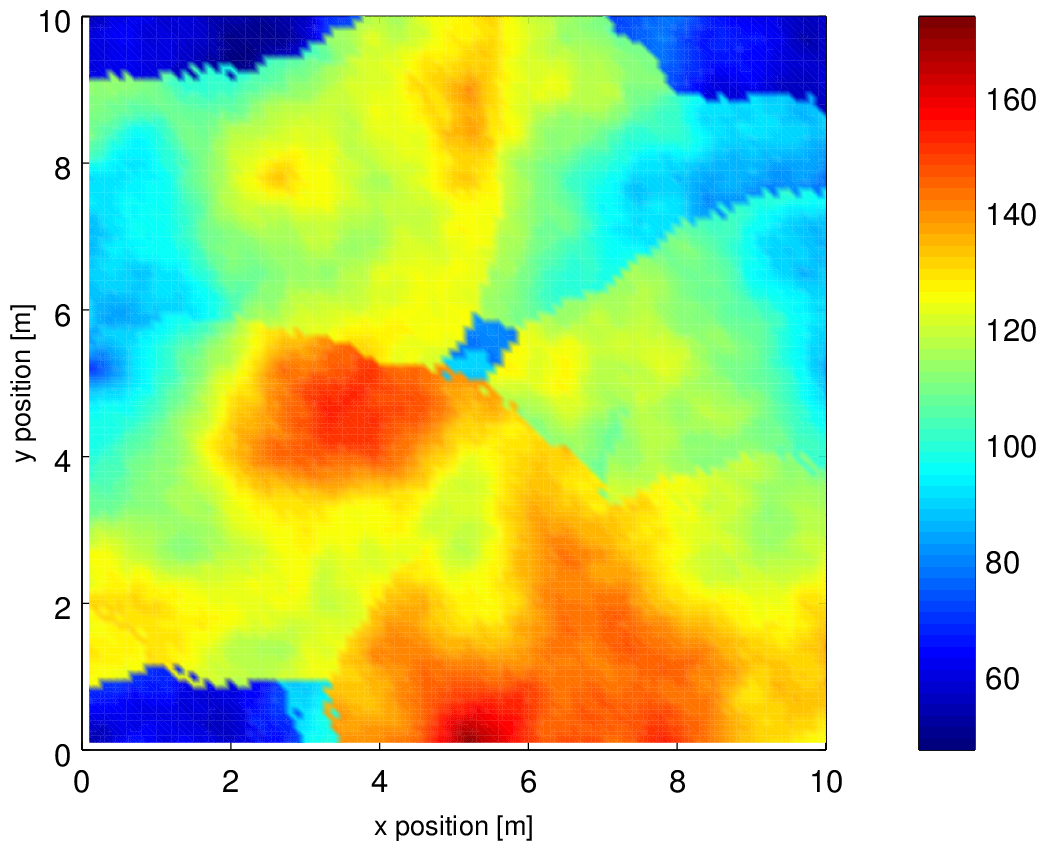
\includegraphics[width=0.24\linewidth]{tasefigs/cost3.png}
    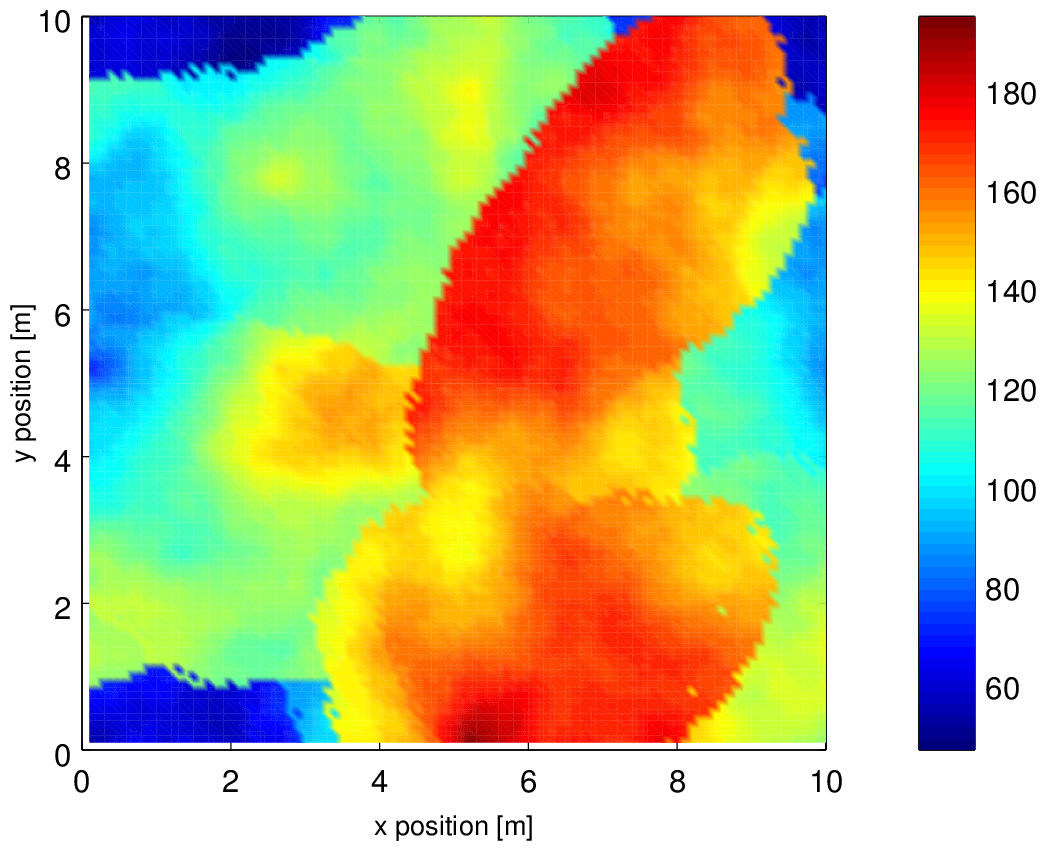
\includegraphics[width=0.24\linewidth]{tasefigs/cost4.png}

    \caption{Shows how the uncertainty surface and the cost surface change
        as the algorithm progresses. These surfaces are used to determine
        the new position of the quadrotors}

    \label{fig:together}

\end{figure}

\begin{figure}[ht]

    \centering
    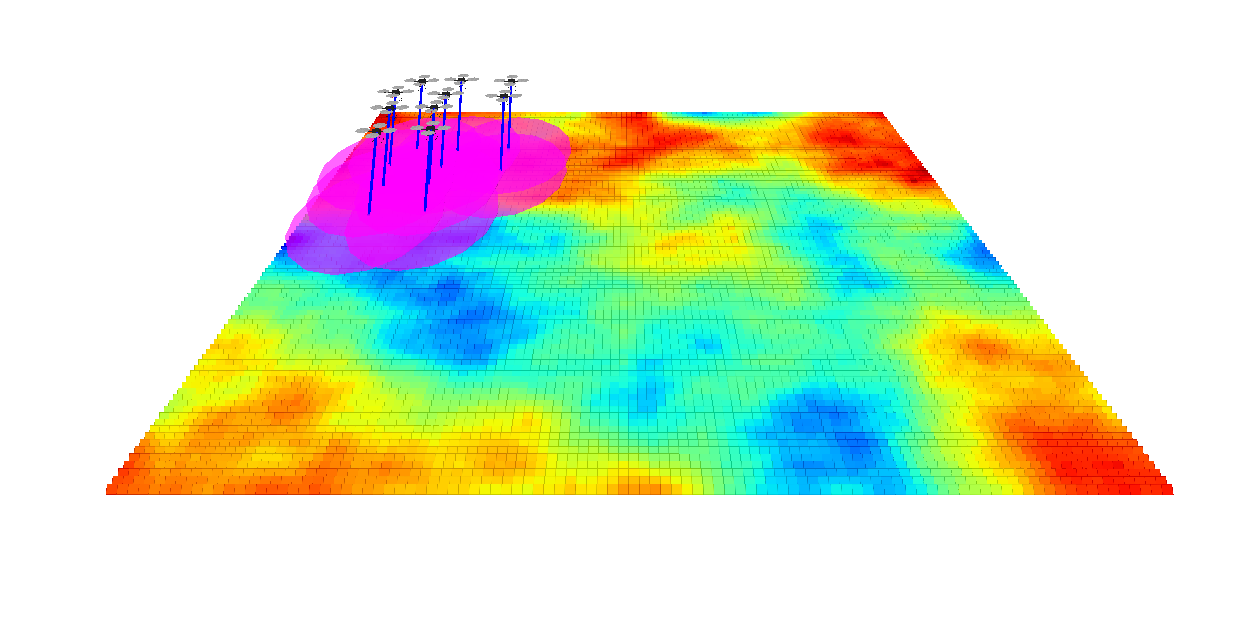
\includegraphics[width=0.24\linewidth]{tasefigs/seq1.png}
    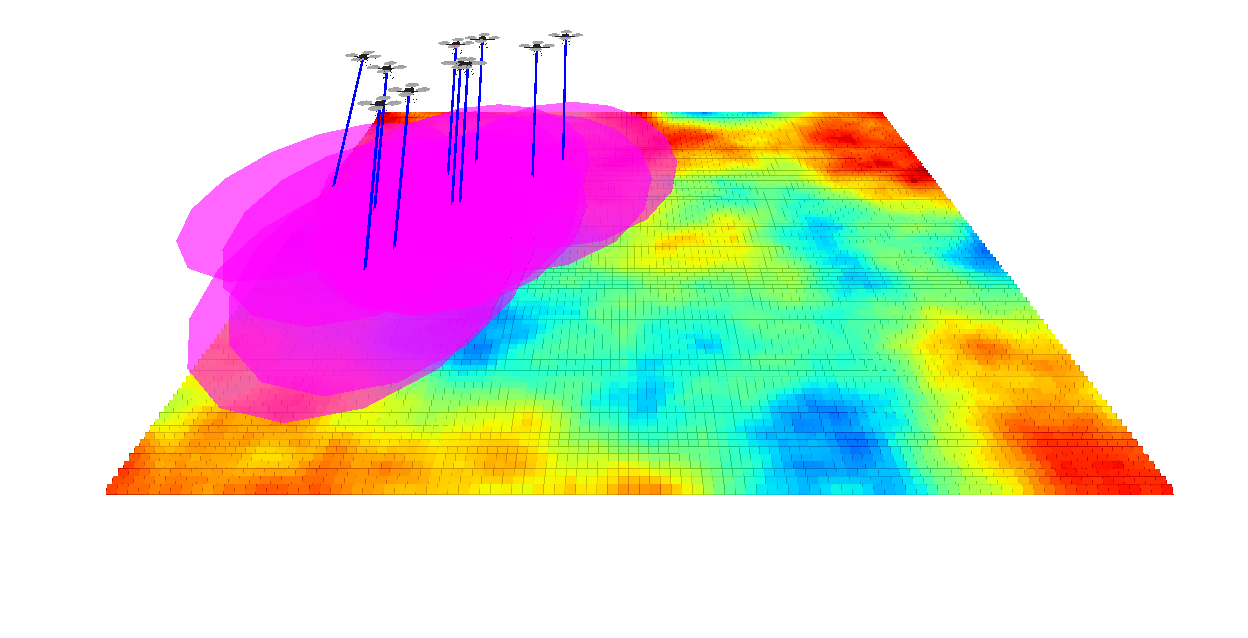
\includegraphics[width=0.24\linewidth]{tasefigs/seq2.png}
    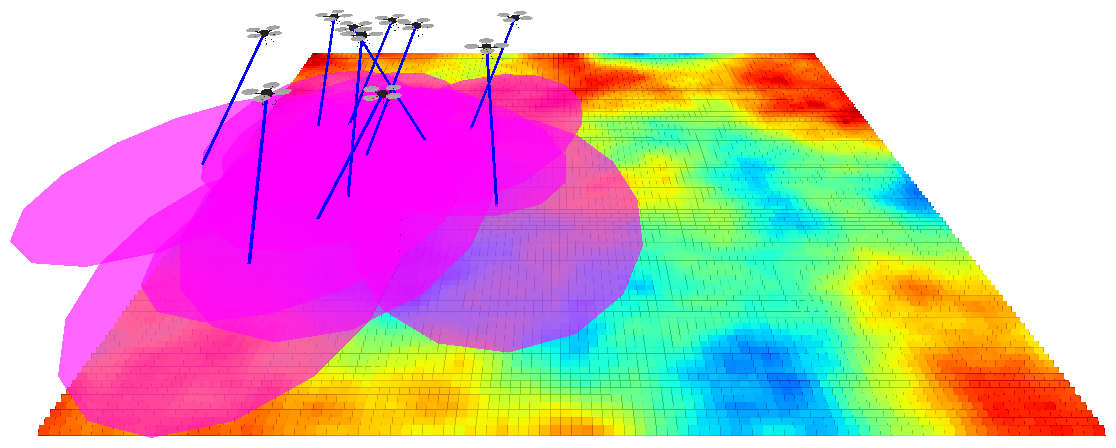
\includegraphics[width=0.24\linewidth]{tasefigs/seq3.png}
    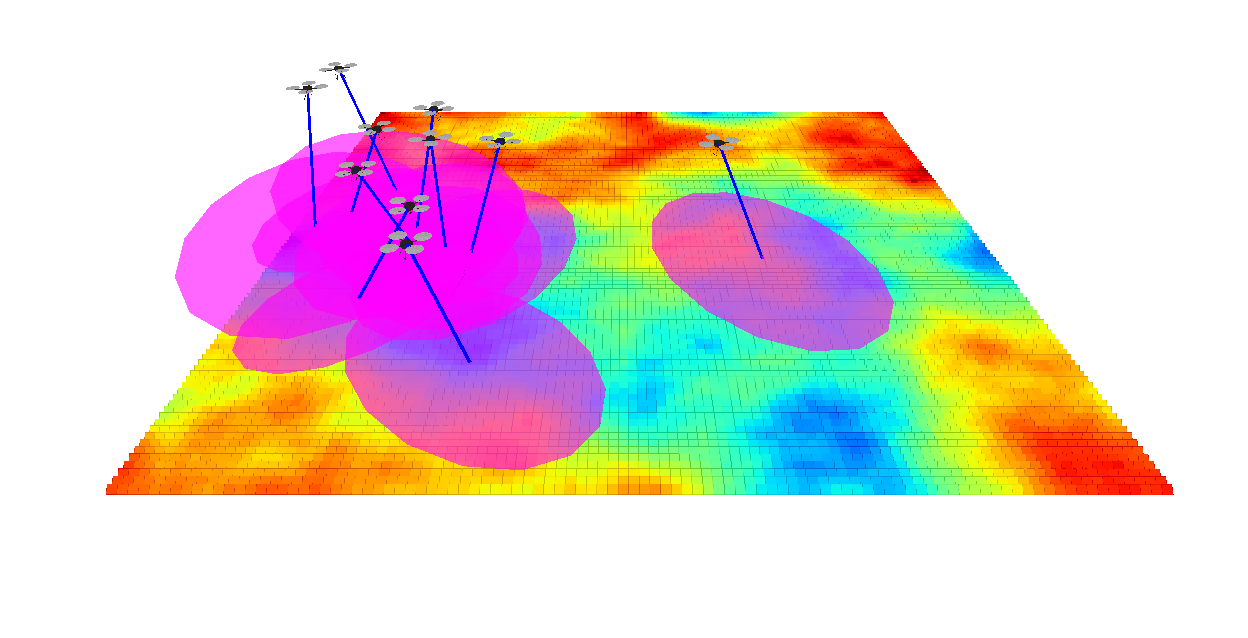
\includegraphics[width=0.24\linewidth]{tasefigs/seq4.png} \\
    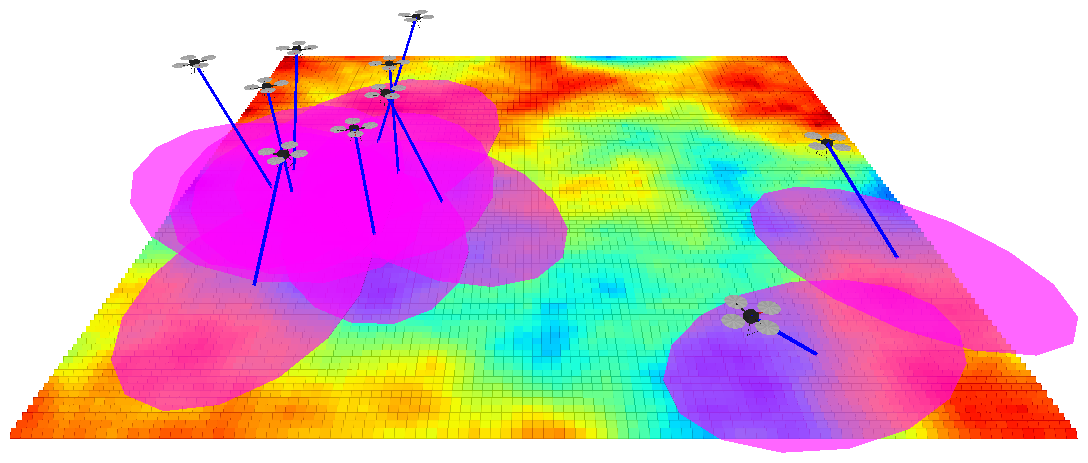
\includegraphics[width=0.24\linewidth]{tasefigs/seq5.png}
    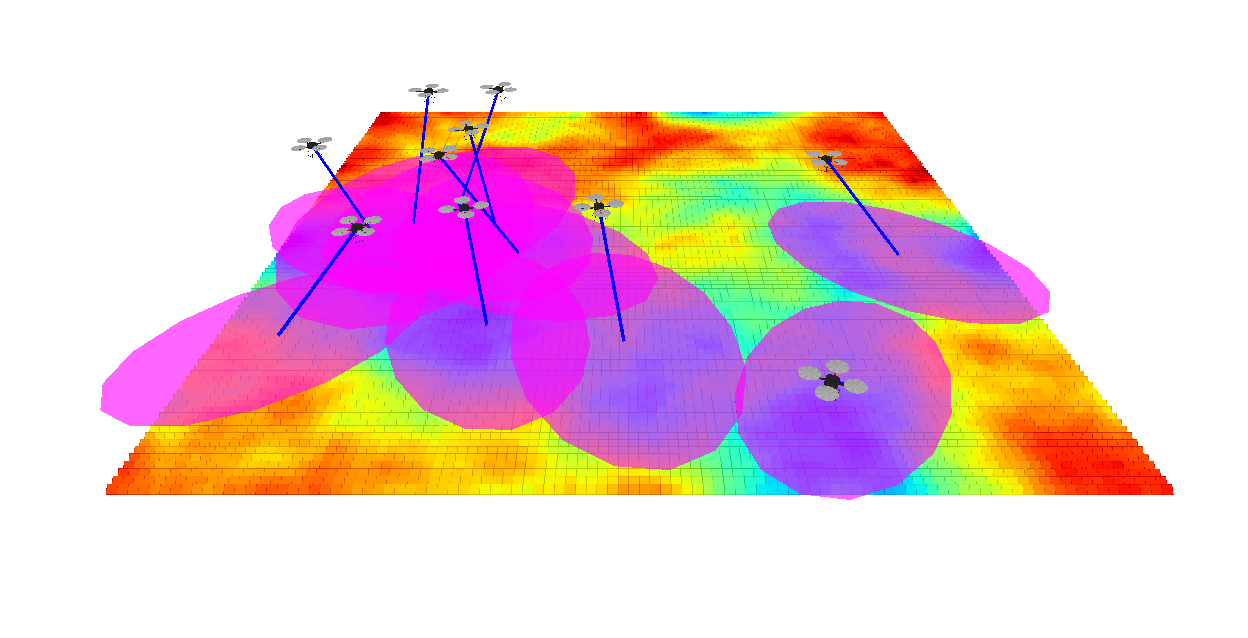
\includegraphics[width=0.24\linewidth]{tasefigs/seq6.png}
    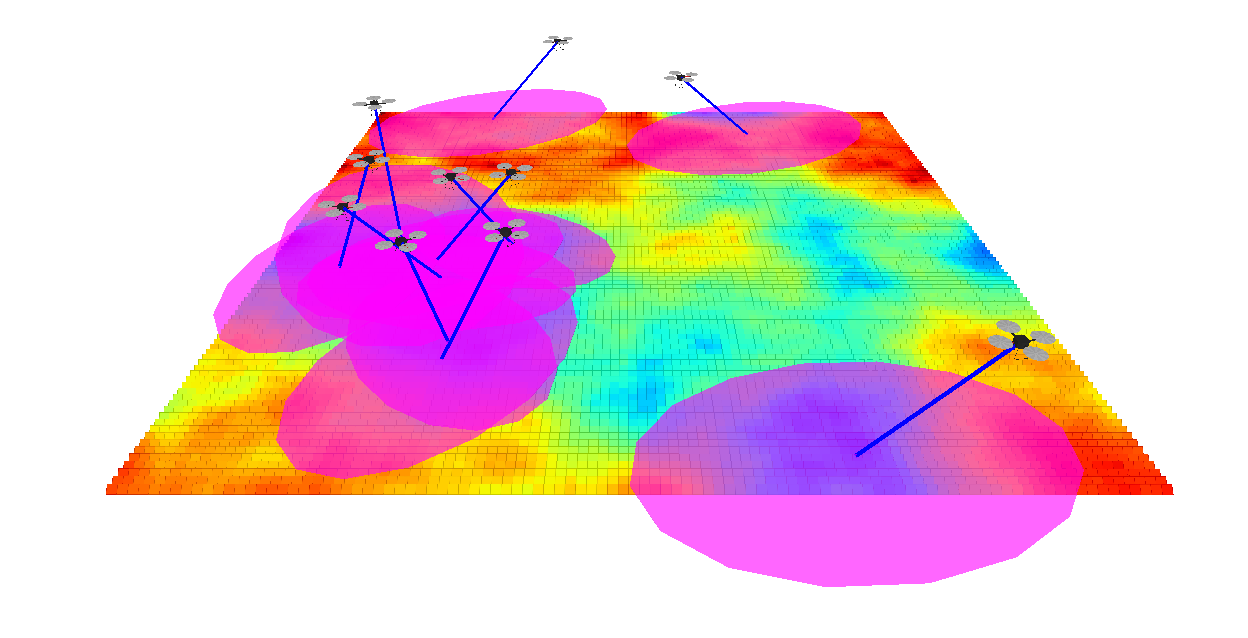
\includegraphics[width=0.24\linewidth]{tasefigs/seq7.png}
    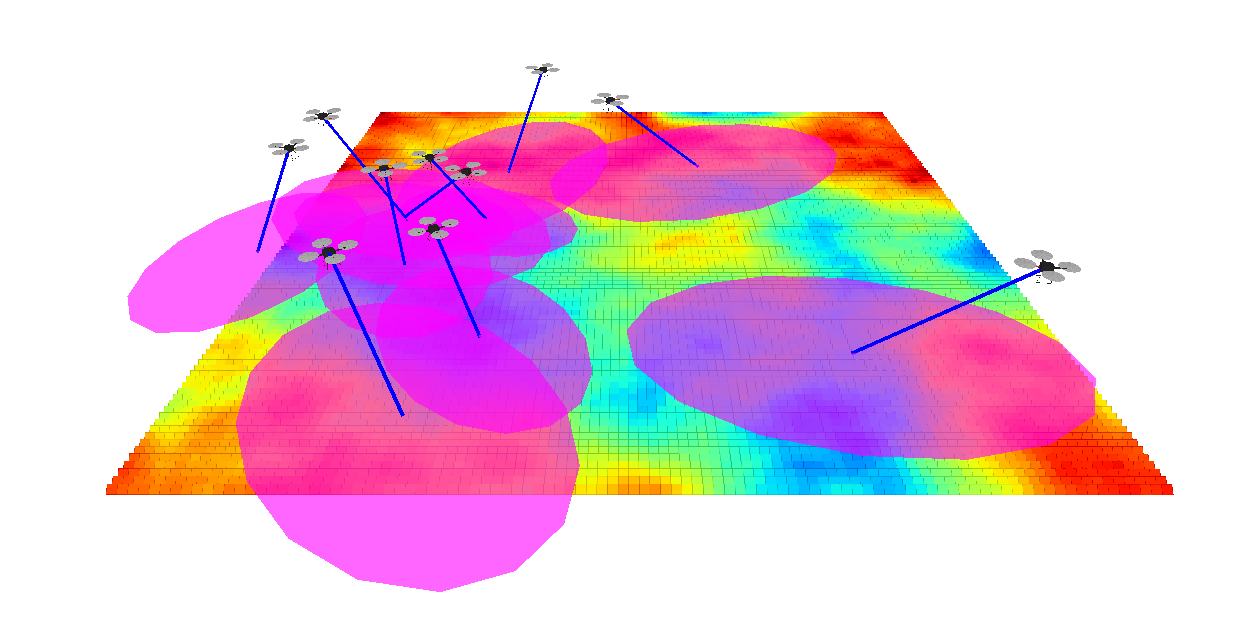
\includegraphics[width=0.24\linewidth]{tasefigs/seq8.png}

    \caption{Shows how the quadrotors move to fill the search space whilst
    trying to avoid the frequency of visit to areas of high risk using 10
    agents}

    \label{fig:seq}

\end{figure}

Fig.~\ref{fig:seq} shows how the quadrotors fill the space whilst reducing the
frequency of visit to high risk areas whilst maintaining persistent coverage
over low risk areas. This figure is a sequence of images that shows how the
algorithm progresses.

\begin{figure}[ht]

    \centering
    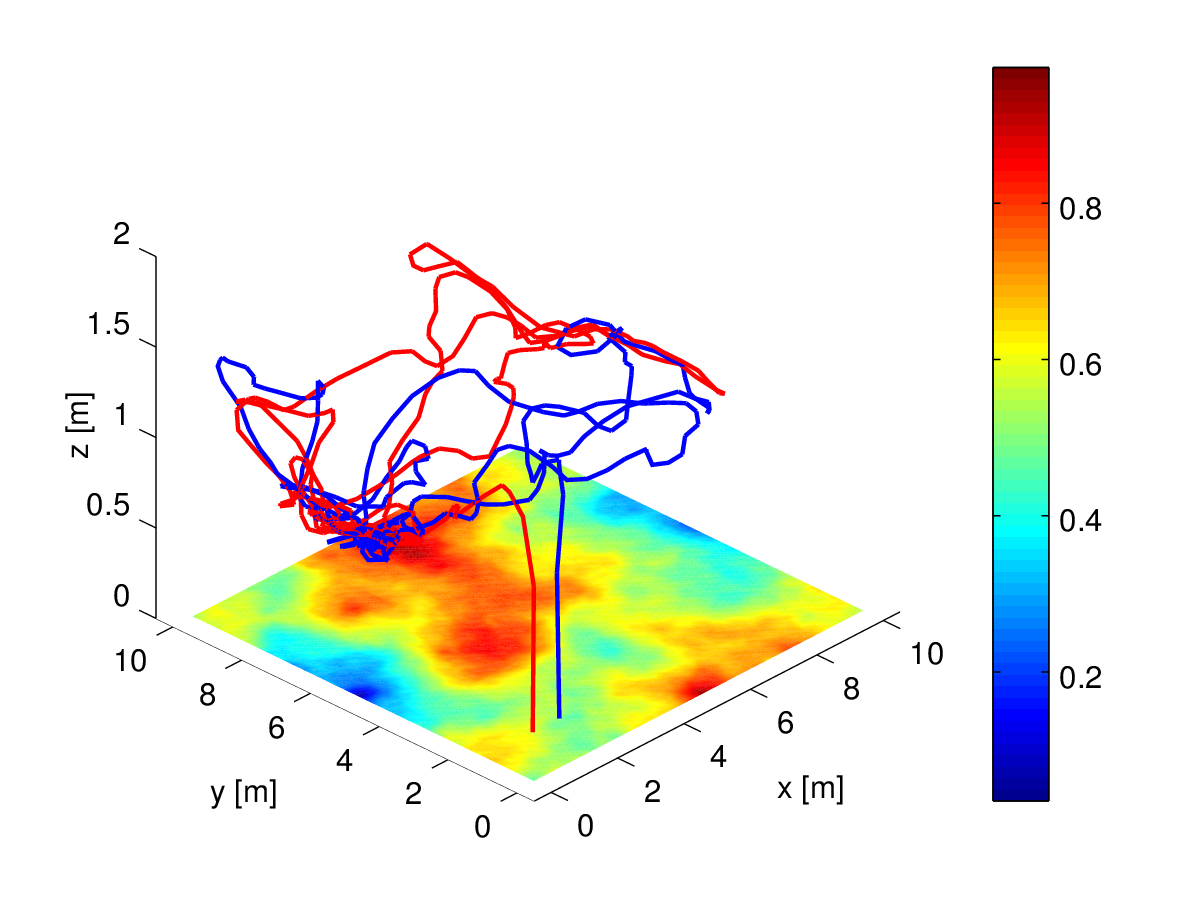
\includegraphics[width=1\linewidth]{tasefigs/trajsim.png}

    \caption{Shows the trajectories of two quadrotors (the red and blue lines)
    performing the algorithm through the search space. Notice that the
    quadrotors stay in low risk areas and increase their height above the
    high risk regions.}

    \label{fig:trajsim}

\end{figure}

\section{Results \& Discussion}

To determine how well Rover performed, we constructed three different
experiments that tested various attributes about the implementation. We have
also gathered four different metrics to show the performance of the
implementation. To gather the experimental data, we decided to use three
different scene sizes. For each of the scene sizes, we used 3 different ground
risk surfaces created using the diamond square algorithm. The experiments
developed are described below and after each description is the associated data
and discussion.

\subsection{Metrics}

The metrics that we are gathering in the experiments are used to show that the
algorithm minimizes risk, maximizes the sensor quality, fills the search space
quickly and persistently, and that the algorithm can be used in a real time
setting. The metrics that are being collected are the average associated risk,
the average associated sensor quality, the average amount of iterations it
takes to reach 90\% cumulative coverage, and the amount of time per iteration.

\subsubsection{Average Associated Risk}

This metric describes the average risk incurred by the quadrotors. Each of
quadrotors is experiencing some sort of risk. By averaging the risk associated
with each of the quadrotors, we are able to quantify how much risk is being
incurred by the swarm. By showing that this metric remains low, indicates that
the algorithm is completing its proposed task.

\subsubsection{Average Associated Sensor Quality}

The average associated sensor quality was acquired by breaking the workspace
into a grid. For each cell in the grid, we record the maximum sensor quality
out of all the quadrotors that are currently viewing that cell. For a unified
metric, we then average all the sensor quality values for all the grid cells
that are currently being covered. This gives an accurate representation of the
average sensor quality for the swarm.

\subsubsection{Persistent Cumulative Coverage}

To show that the proposed approach persistently covers the search area, we
gathered the number of iterations for the algorithm to reach 90\% cumulative
coverage throughout progression of each run. This means that once the algorithm
reached 90\% cumulative coverage, we recorded the number of iterations it took,
and reset the cumulative coverage back to zero. We then averaged the number of
iterations it took. This is a good metric for showing persistent coverage
because it captures how long it takes for the agents to fill the space from
many different initial configurations. If there is a low deviation between the
values, then we know that the initial configurations of the quadrotors had
little to no effect on the persistence of coverage. Also, this metric can be
used to to determine how quickly the quadrotors filled the area on average.
This becomes the standard performance metric used for the algorithm.

\subsubsection{Time per Iteration}

Since this algorithm is to be used in a real-time setting, we need to show that
each iteration (or each update of the quadrotors' positions) shouldn't take too
long. This metric shows the feasibility of the approach in a real-time
scenario.

\subsection{Performance as function of the number of quadrotors}

To determine the performance as a function of the number of quadrotors in the
swarm, we ran the algorithm for 1000 iterations on each of the nine scenes
using a swarm size of $1, 5, 10, \cdots, 35$. The purpose of this experiment is
to show that the algorithm scales gracefully as the number of quadrotors used
in the swarm increases. The average risk, average sensor quality, and average
number of iterations between 90\% cumulative coverage were collected to show
how the algorithm scales as the number of quadrotors increases.

Fig.~\ref{fig:nqs_r_sq} shows the average risk and sensor quality for the swarm
as the number of quadrotors increased. For the graph, we averaged the average
risk for each of the three scenes for each of the scene sizes. This allows us
to get a better picture of the trend as the number of quadrotors increases.
Fig.~\ref{fig:nqs_r_sq} shows the number of quadrotors has little effect on the
average associated risk and average sensor quality. We also see that the size
of the scene has little effect on these metrics. The figure shows that the
average associated risk is under 0.1 (10\% risk) for any number of quadrotors
and that the average sensor quality is over 0.6 (60\% sensor quality) for any
number of quadrotors. Therefore, the algorithm is meeting two of the three
prescribed task, maintaining high sensor quality whilst maintaining low risk.

\begin{figure}[h!]

    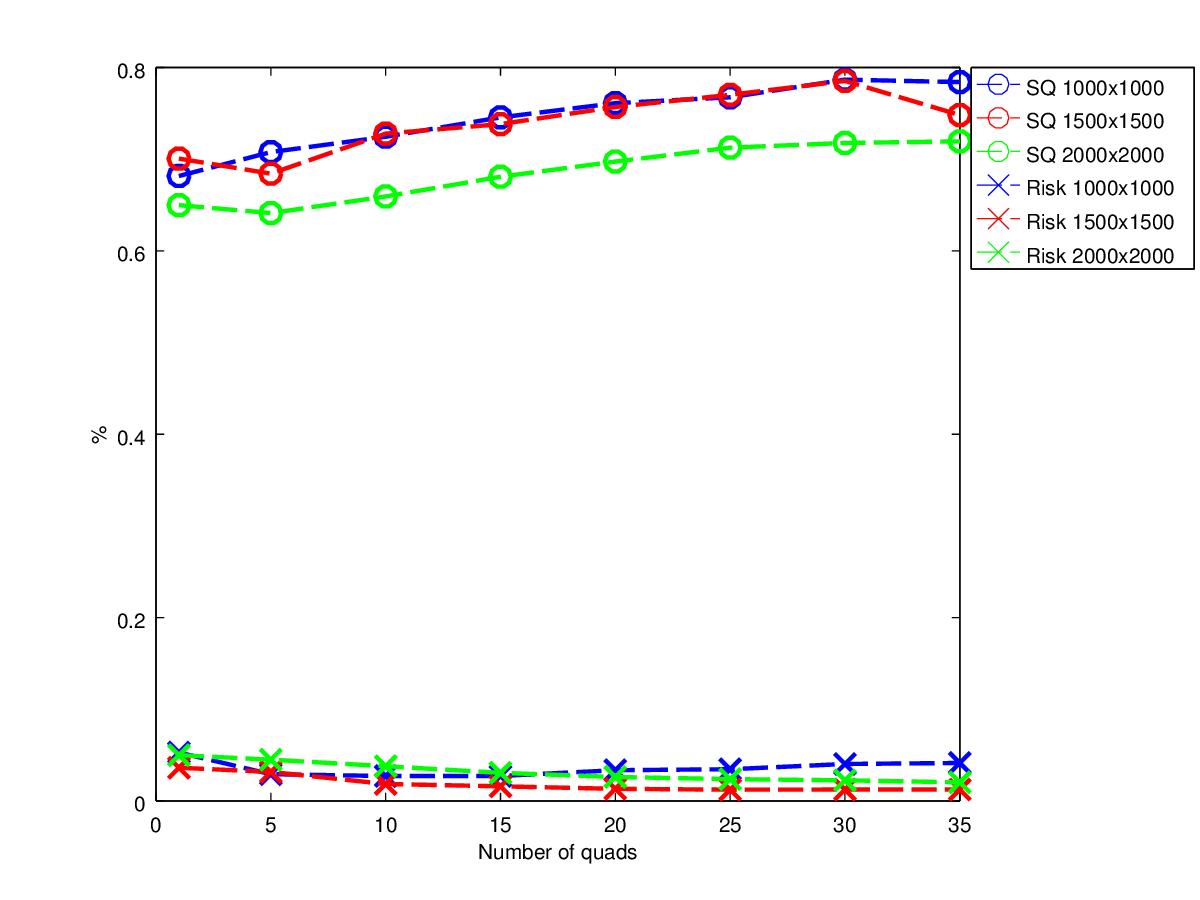
\includegraphics[width=1\columnwidth]{tasefigs/perf_quads_sq_risk.png}

    \caption{Figure showing how risk and sensor quality relate to the number of
    quadrotors}

    \label{fig:nqs_r_sq}

\end{figure}

\begin{figure}[h!]

    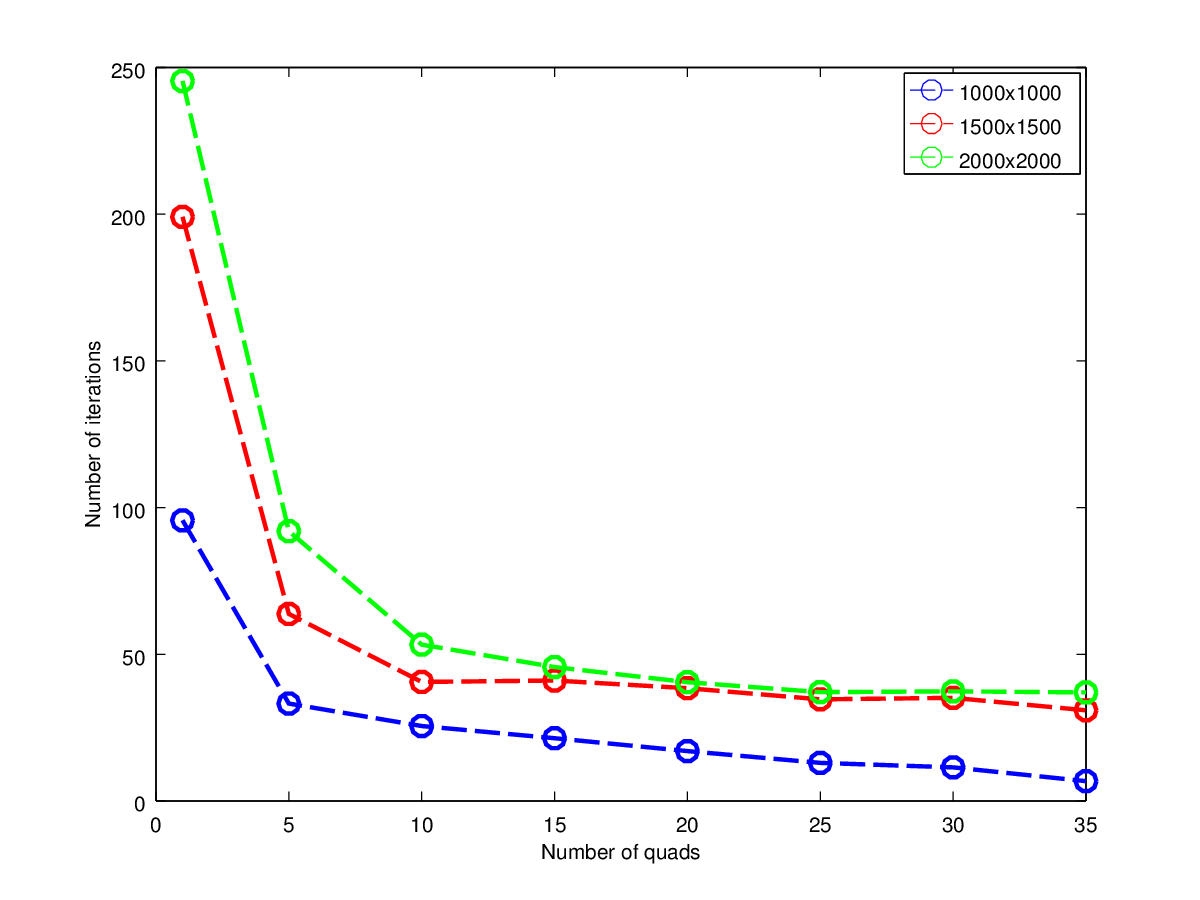
\includegraphics[width=1\columnwidth]{tasefigs/perf_quads.png}

    \caption{Figure showing the average number of iterations needed to reach
        90\% cumulative coverage}

    \label{fig:nqs_cum}

\end{figure}

We also needed to quantify the persistence of the coverage as the number of
quadrotors increased. This is shown in Fig.~\ref{fig:nqs_cum}. We can see that
average number of iterations it takes for the algorithm to reach 90\%
cumulative coverage decreases exponentially as the number of quadrotors
increases then converges. We also see that the algorithm fills the area more
quickly for smaller scene sizes, as expected. The graph shows that the
algorithm is able to provide persistent coverage over a given area. To give
some context for this graph, if the average cumulative convergence metric was
100 iterations for 5 quadrotors on a 20m by 20m area and it takes 0.5s per
iteration and we run the algorithm for 750 iterations, the quadrotors reach
90\% cumulative coverage 7.5 times over this 400~$m^2$ area. On average it
takes 50s to reach this 90\% convergence. Also keep in mind that the speed of
the quadrotors was capped at 0.4 meters per iteration, or in this case, 0.8
meters per second. This quick convergence combined with the data from
Fig.~\ref{fig:nqs_r_sq} shows that the algorithm is able to maintain persistent
coverage of the area whilst maintaining low risk and high sensor quality.

\subsection{Performance as a function of control noise}

In order to determine if the algorithm would be able to withstand an acceptable
amount of error in the controller, we have conducted experiments to test the
performance by changing the amount of noise that is present in the simulated
proportional-integral-derivative (PID) controller. We did this by adding
Gaussian noise to the control output of the PID controller. The noise was
quantified by altering the standard deviation of the Gaussian function. For the
experiments, the mean for the Gaussian was set to zero and the standard
deviation was set from 0 to 0.6 meters with a step of 0.2 meters. This range of
values seemed to be an accurate representation of the control noise present on
the AscTec Pelicans we used for the practical experimentation. For the
experiments, only one scene size was used ($1500 \times 1500$) but three
different scenes of that size were used. The number of quads used was 10, 20,
and 30 which gave a good overall depiction of the algorithm. The resultant
performance information was gathered and averaged. Fig.~\ref{fig:res_cn_r_sq}
shows trends for the three different swarm sizes that were used and how the
control noise affected the risk and sensor quality.

\begin{figure}[h!]

    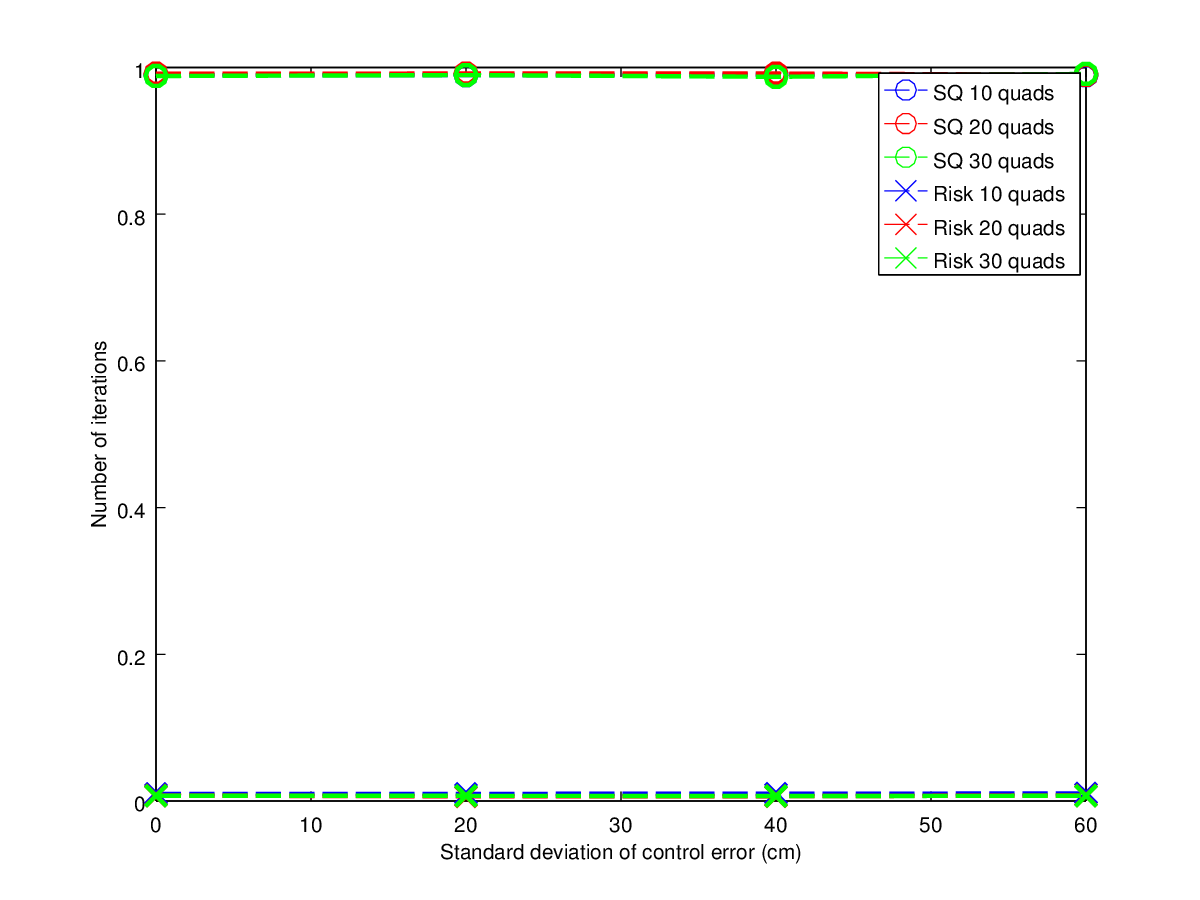
\includegraphics[width=1\columnwidth]{tasefigs/cn_sq_risk.png}

    \caption{The trend shows how the control noise can affect the risk and
        sensor quality performance of the algorithm for different swarm sizes}

    \label{fig:res_cn_r_sq}

\end{figure}

Fig.~\ref{fig:res_cn_r_sq} shows that the control noise does not affect the
performance of the algorithm in terms of the associated sensor quality and
risk. Since the algorithm is purely reactive, we can see that within an
acceptable amount of noise, that the algorithm is still able to perform well
based on the metrics we have used.

\begin{figure}

    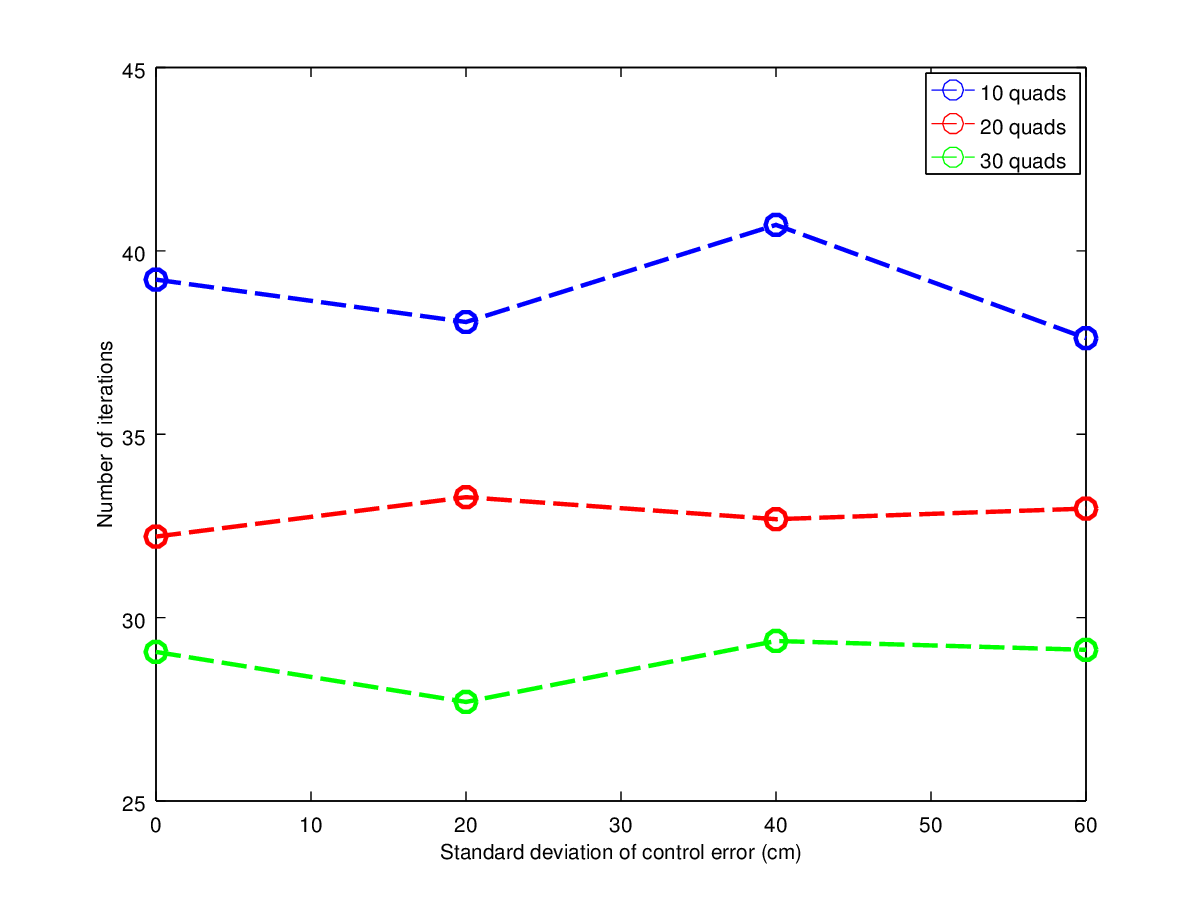
\includegraphics[width=1\columnwidth]{tasefigs/perf_cn.png}

    \caption{The trend shows how the control noise affects the cumulative
    coverage rate}

    \label{fig:res_perf_cn}

\end{figure}

Fig.~\ref{fig:res_perf_cn} shows that the control noise does not affect the how
persistent the coverage is. This is yet another benefit of the algorithm being
purely reactive.

\subsection{Computational Efficiency}

\begin{figure}[h!]

    \centering
    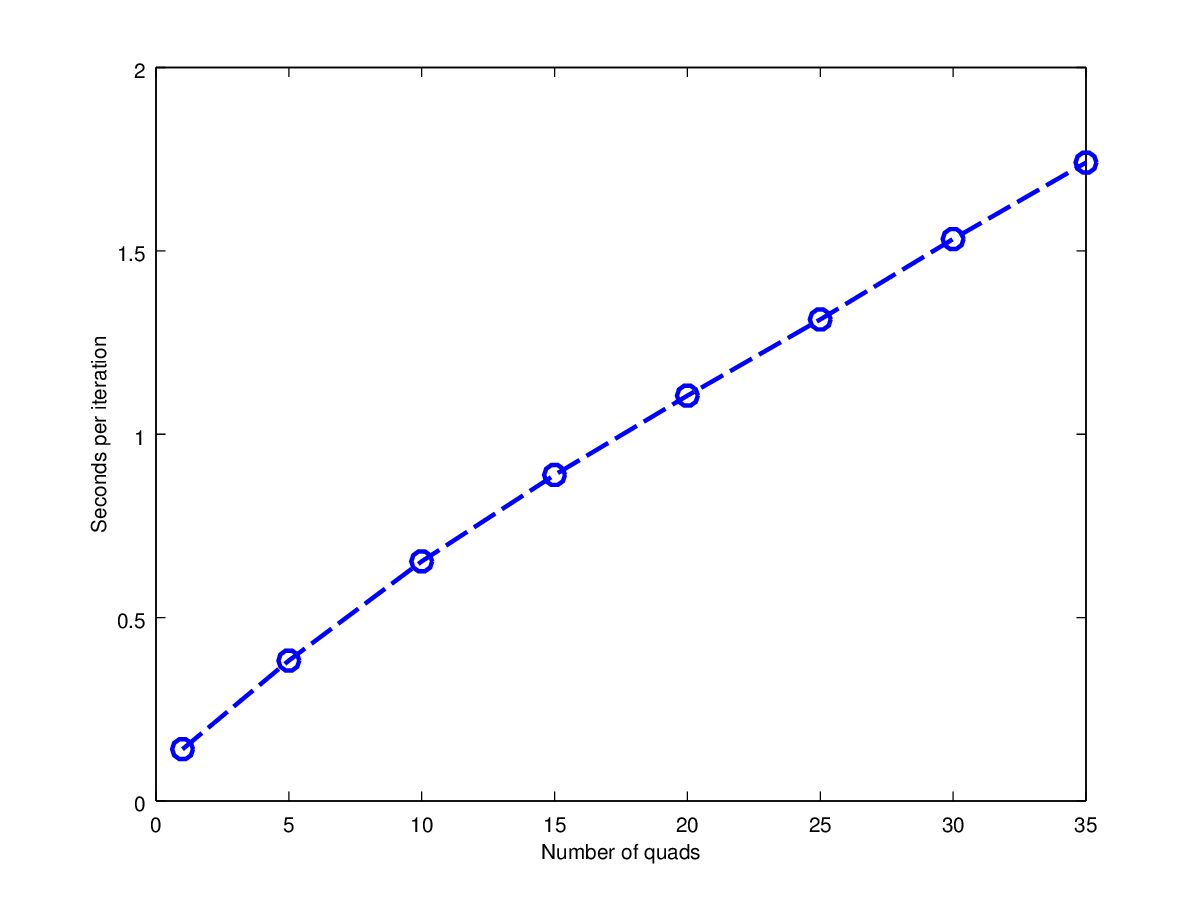
\includegraphics[width=0.49\columnwidth]{tasefigs/comp_eff.png}
    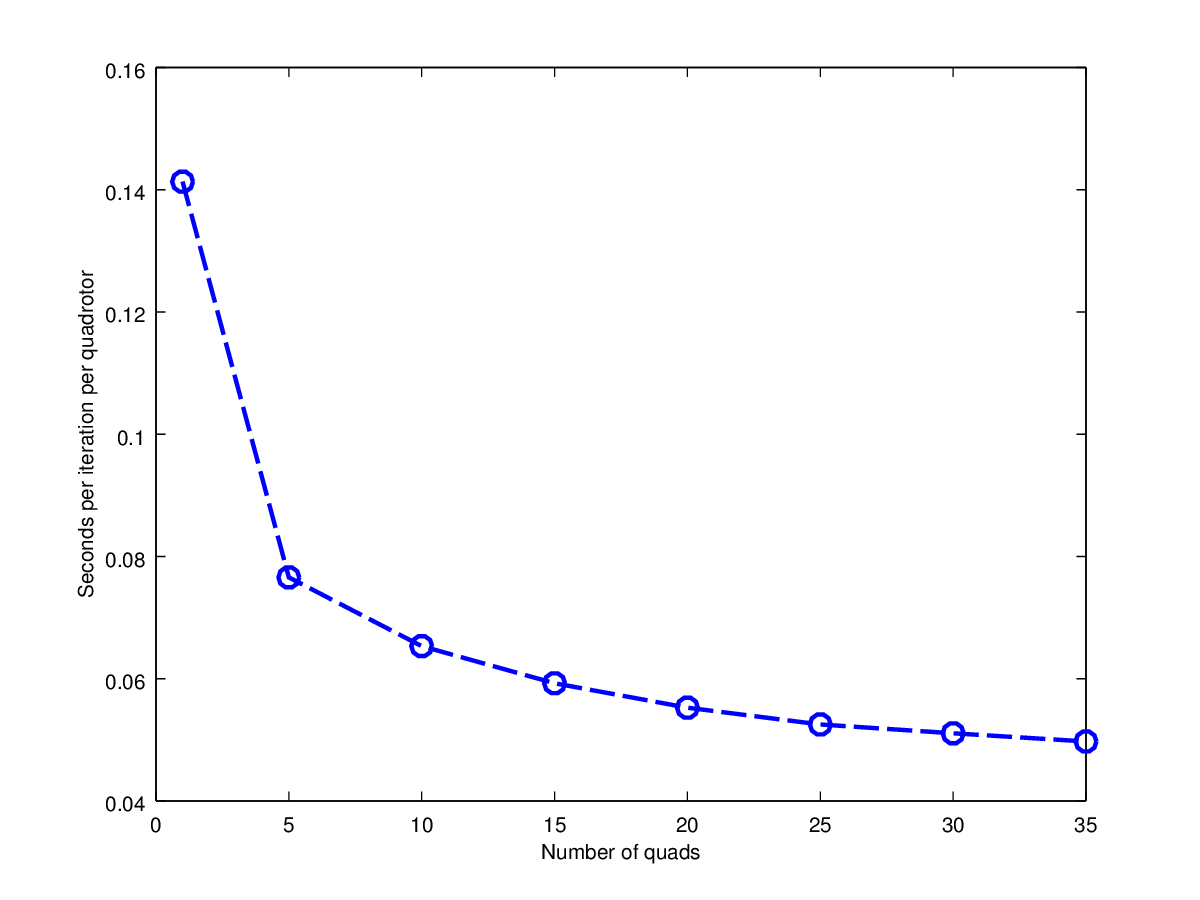
\includegraphics[width=0.49\columnwidth]{tasefigs/comp_eff_per_quad.png}

    \caption{The first figure shows how the amount of time per iteration
    increases as the number of quadrotors in the swarm increases. The
    second figure shows how the amount of time per iteration per quadrotor
    changes as a function of the number of quadrotors.}

    \label{fig:comp_eff}

\end{figure}

In order to show that the algorithm can run in a real-time scenario we have
graphed the how long each iteration takes to execute as a function as the size
of the swarm increases. The figure on the left in Fig.~\ref{fig:comp_eff} shows
this trend.  We see a linear increase in the amount of time to plan every the
entire swarm for each iteration. The figure on the right in
Fig.~\ref{fig:comp_eff} shows how the time per iteration per quadrotor
increases as the number of quads in the swarm increases. We see that if we used
a decentralized approach, the amount of time per iteration becomes quite
manageable.

\subsection{Practical Experiments}

We tested the algorithm at the Laboratory for Autonomous Systems Research
located at the Naval Research Laboratory in Washington DC\@. We used two AscTec
Pelican quadrotors that were operated in a 5.2 meter by 5.2 meter area
surrounded by 10 Vicon motion capture cameras. The quadrotors were equipped
with with passive motion capture markers which were seen by the Vicon cameras.
The Vicon cameras have LEDs which were used to illuminate the passive markers.
The 3D positions and the orientations of the quadrotors were sent to a laptop
which uses the Robotic Operating System (ROS) and a swarm middleware called
ZeroMQ-ROS to compute the control commands and to send them to the vehicles.
ROS is a open-source middleware combined with software libraries and tools to
build robotic applications. ZeroMQ-ROS is a middleware for controlling a swarm
using a ROS multi-master architecture. The control commands were sent over WiFi
through a socket to each of the quadrotors.

\begin{figure}[ht]

    \centering
    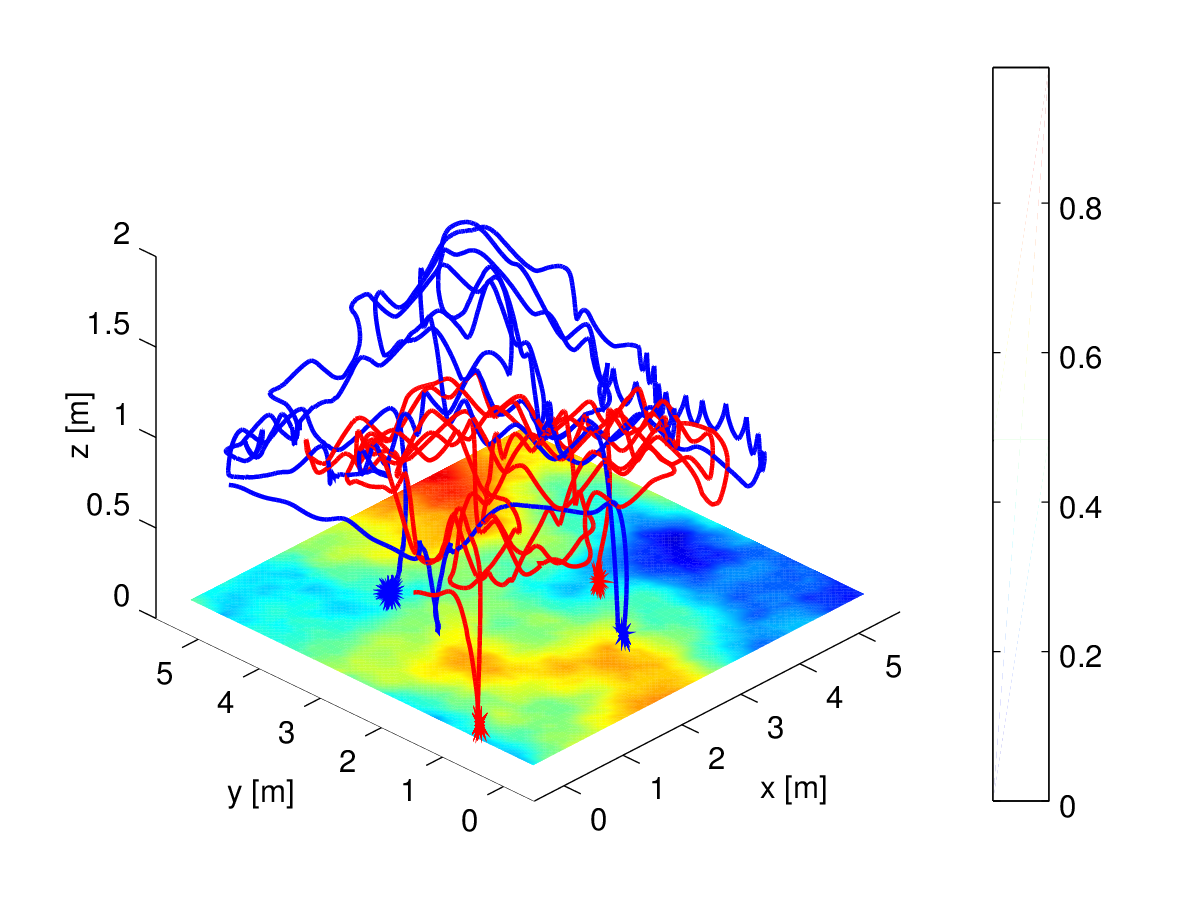
\includegraphics[width=1\columnwidth]{tasefigs/trajpractical.png}

    \caption{Shows the trajectories for the practical experiments that were
        run using the AscTec Pelicans at the Laboratory for Autonomous Systems
    Research at the Naval Research Laboratory. The oscillations shown are
    caused by the control noise.}

\end{figure}

\bibliographystyle{IEEEtran} \bibliography{mp,plaku,quads,relatedwork}

\end{document}
